\documentclass[a4paper,12pt]{article}

% Packages
\usepackage{amsmath}
\usepackage{geometry}
\usepackage{enumitem}
\usepackage{hyperref}
\usepackage{parskip}
\usepackage{graphicx}
\setlength{\parindent}{0pt}

% Page layout settings
\geometry{left=2.2cm, right=2.2cm, top=2.2cm, bottom=2.5cm}

\title{\vspace{-1cm}\Huge{ASTR4004/ASTR8004 2026\\Astronomical Computing Assignment 2}}
\author{Sven Buder}
\date{\textbf{due Thursday, 3 September, 2026}}

\begin{document}

\maketitle

This assignment is worth \textbf{20 points}. All necessary files can be found at \url{https://github.com/svenbuder/astro_comp_assignment02_2026} and its \texttt{data/} directory.

Complete the analysis in Jupyter notebooks and upload all code/notebooks and figures to your GitHub repository. Add Markdown cells for short explanations and answers. Figures should be clearly labelled and suitable for communicating your results to another astronomer.

Tasks with a $\star$ are intended to distinguish strong submissions. The task with $\star\star$ is intended to be the most difficult and time-intense task.

\textbf{Manage your time.} Some parts of this assignment can be completed quickly, while others invite more experimentation. The number of marks available should guide how much time you invest: a robust partial solution that allows you to continue with the rest of the assignment can be preferable to spending hours perfecting one difficult step.


\section{\texttt{git} in Practice \hfill [2 points]}

Being able to share code and collaborate on projects is essential in both astronomical research and data science. Use a GitHub repository to track your work throughout this assignment.

Demonstrate that you can:

\begin{itemize}
    \item initialise a repository and push content to the \textit{main} branch;
    \item create and work on a branch with a descriptive name;
    \item make regular commits with meaningful commit messages;
    \item merge your branch back into \textit{main}.
\end{itemize}

Maintain a clear directory structure, with data in \texttt{data/} and figures in \texttt{figures/}.

Submit the link to your GitHub repository and specify your main working branch if it differs from \textit{main}.


\section{Bright Stars Around M67 with ADQL \hfill [6 points]}

A colleague is interested in the open cluster Messier 67 (RA = 132.825 deg, Dec = 11.8 deg) and is considering an observation proposal using the 2dF fibre positioner and HERMES spectrograph (effective for Gaia $G<14$) to follow up stars observed with the APOGEE spectrograph, for which they only have 2MASS catalogue identifiers.

Your task is to assist by querying Gaia DR3 and performing some basic analysis.

\begin{enumerate}[leftmargin=0.7cm]

    \item Write an ADQL query that returns all stars in the Gaia DR3 \texttt{gaiadr3.gaia\_source} table within $1$ degree of M67 with $G<14$ (\texttt{phot\_g\_mean\_mag}) and crossmatches them with 2MASS (\texttt{gaiadr1.tmass\_original\_valid}). You can execute the query on the Gaia archive website or via \textsc{astroquery}. Include your ADQL query in the notebook and report the number of returned stars.

    \item Identify stars with:
    \begin{itemize}
        \item bad 2MASS photometry (\texttt{ph\_qual} is not \texttt{'AAA'});
        \item non-positive values of Gaia \texttt{parallax}.
    \end{itemize}
    Apply these quality cuts and report how many stars remain.

    \item Create and save a two-panel figure showing:
    \begin{itemize}
        \item Gaia BP$-$RP versus absolute $G$ magnitude, using \texttt{bp\_rp};
        \item 2MASS J$-$Ks versus apparent $H$ magnitude, using
        \texttt{j\_m}, \texttt{h\_m}, and \texttt{ks\_m}.
    \end{itemize}

    \item $\star$ Based only on fibre usage, would you recommend this field for a 2dF/HERMES observing proposal? Support your answer quantitatively.

\end{enumerate}


\section{Radial Metallicity Relations in Simulations \hfill [6 pts]}

The radial metallicity relation describes the change of metallicity -- here the gas-phase metallicity $\mathrm{A(O)}=\log_{10}(N_\mathrm{O}/N_\mathrm{H})+12$ -- with galactocentric cylindrical radius $R_\mathrm{Gal.}$. Radial metallicity gradients provide insight into processes such as inside-out formation, gas accretion, outflows, and radial migration. A lot of work has been done through observational studies (e.g. Ho et al., 2017, ApJ, 846, 39) and a few simulations (e.g. Grand et al., 2016, MNRAS, 460, 94), but more works is needed to understand variations of the radial metallicity gradient.

Your colleague has completed a cosmological simulation of a Milky-Way-like spiral galaxy. The FITS file \texttt{data/nihao\_uhd\_simulation\_g8.26e11\_xyz\_positions\_and\_oxygen\_ao.fits} contains the gas-phase metallicity $\mathrm{A(O)}$ and $(x,y,z)$ positions of gas particles within $R_\mathrm{Gal.} = \sqrt{x^2 + y^2} <25\,\mathrm{kpc}$.
Perform the following tasks and save your figures in \texttt{figures/}:

\begin{enumerate}[leftmargin=0.7cm]

\item Plot a two-panel figure:
    \begin{itemize}
        \item (a) logarithmic density plot of $R_\mathrm{Gal.}$ vs. $\mathrm{A(O)}$, with a linear fit and legend;
        \item (b) residuals of the fit, $R_\mathrm{Gal.}$ vs. $\Delta\mathrm{A(O)}$.
    \end{itemize}

\item Use a \texttt{python} fitting tool to fit a linear function to the data, reporting the intercept and slope with uncertainties. Include any hyperparameters used.

\item $\star$ Discuss where the linear model fits well and where it does not. Use statistical metrics, such as the root mean square or another goodness-of-fit indicator, to quantify its performance overall and in regions with larger residuals.

\item Plot a three-panel figure for the $x$ vs. $y$ plane using the same bins and sensible colormaps:
    \begin{itemize}
        \item (a) 2D histogram of the median simulated $\mathrm{A(O)}$;
        \item (b) 2D histogram of the median fitted $\mathrm{A(O)}$;
        \item (c) 2D histogram of the median residuals
        $\Delta\mathrm{A(O)}$.
    \end{itemize}

\item Describe your choice of 2D bins. Discuss what details would be missed with fewer bins and what problems could arise with more bins.

\item $\star$ Analyse the residuals in more detail and propose a reasonable physical explanation for any patterns you observe.

\end{enumerate}

\section{Stellar Spectrum Reduction \hfill [6 points]}

Veloce is a high-resolution echelle spectrograph. The
\texttt{flat.fits} and \texttt{moon.fits} in \texttt{data/} contain the same
$4112\times385$ pixel detector region around the Ca\,II triplet
($\sim851$--$871\,\mathrm{nm}$).

\vspace{-0.5cm}
\begin{figure}[h!]
    \centering
    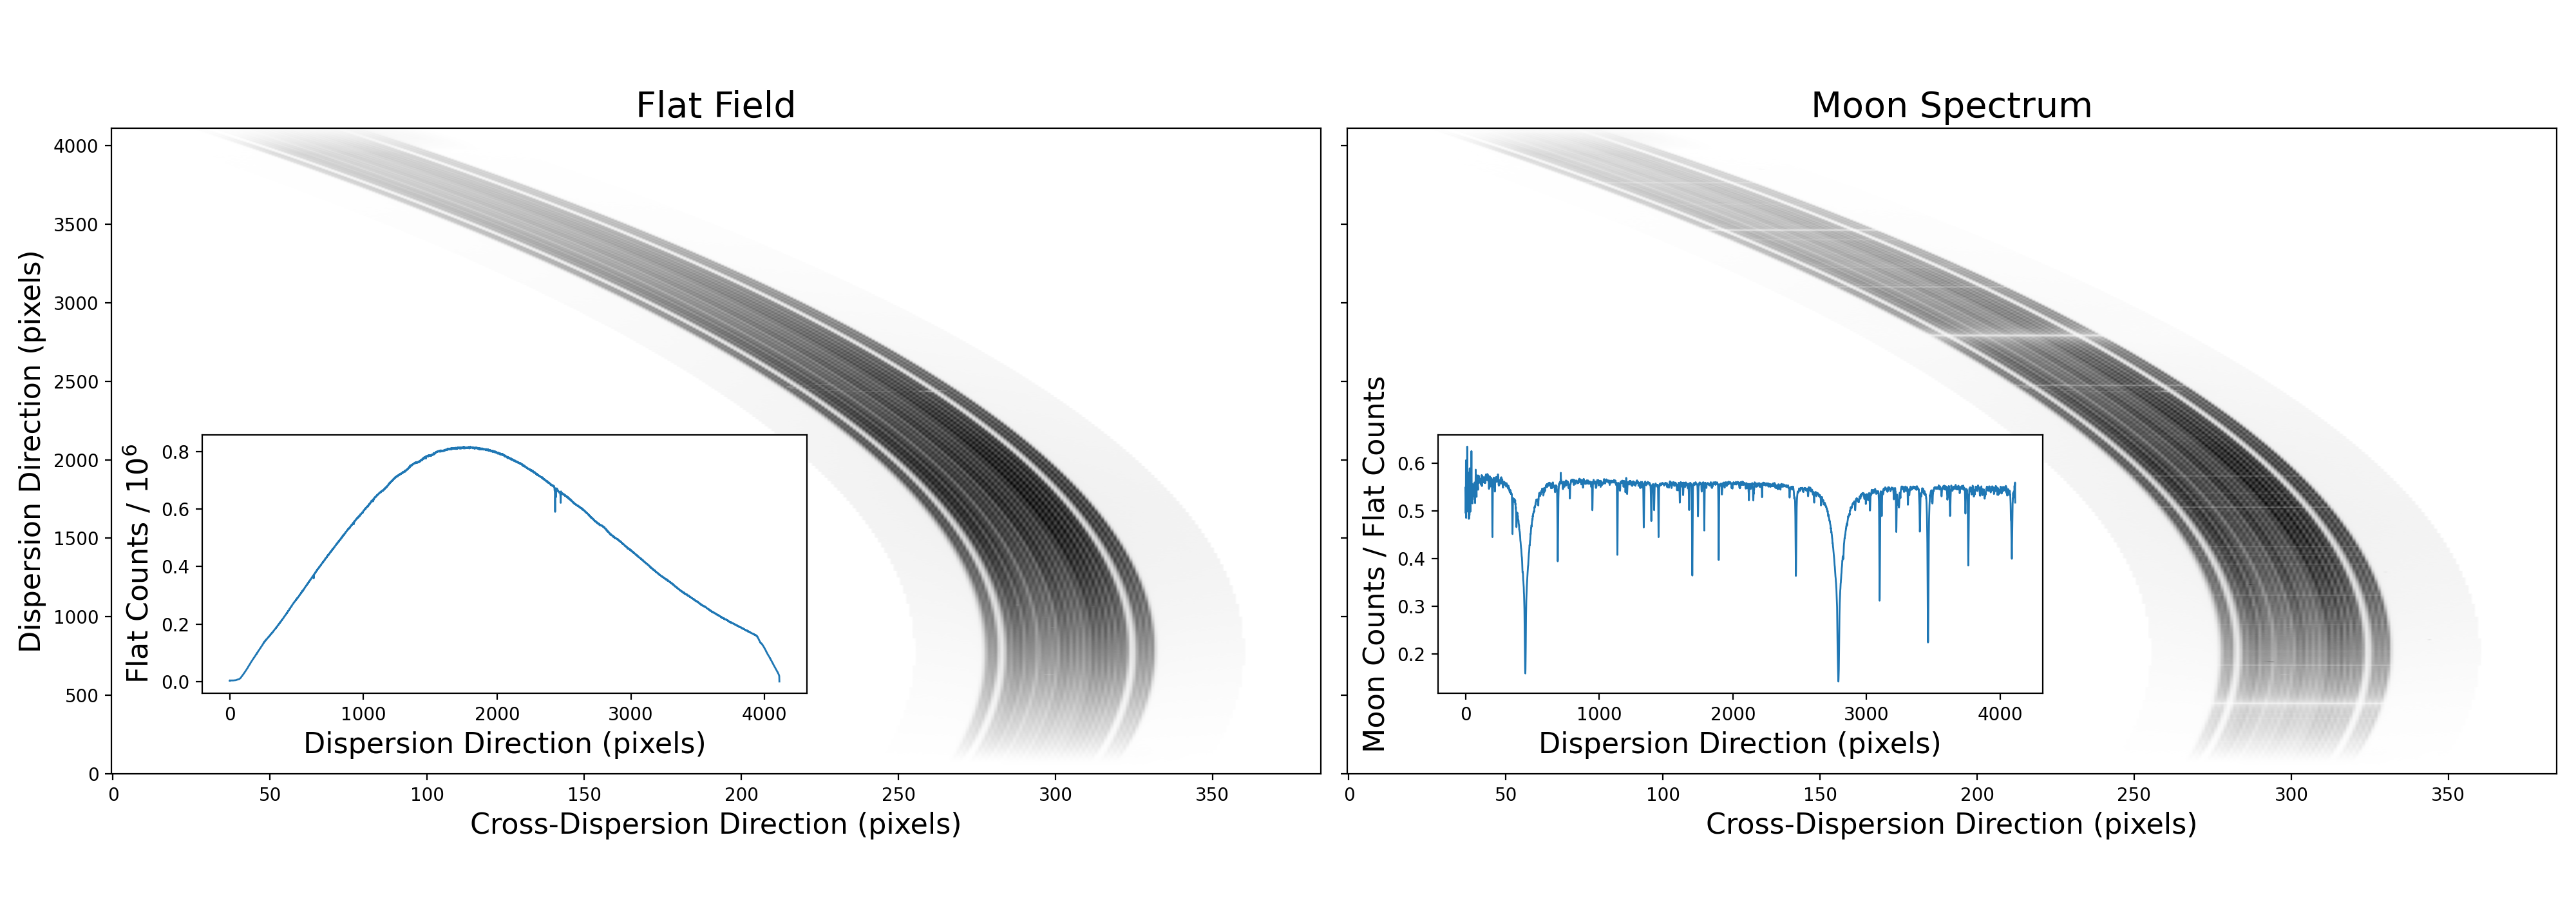
\includegraphics[width=\textwidth]{figures/veloce_flat_moon_cutouts.png}
    \caption{Veloce flat-field (left) and Moon (right) cut-outs. The insets
    show a simple cross-dispersion sum of the flat and the corresponding
    Moon/flat ratio.}
    \label{fig:veloce_cutouts}
\end{figure}

The dispersion direction is vertical and the cross-dispersion direction
horizontal. The central science fibres are bounded by two low-illumination
gaps; the curves following these gaps are the \textit{tramlines}. Signal from
neighbouring spectral orders has been set to zero. You may assume that the
distance between the two tramlines is constant.

\begin{enumerate}[leftmargin=0.7cm]

    \item $\star\star$ \textbf{Determine the tramlines. \hfill [2 points]}

    Use the flat-field image to determine the tramline positions as a function
    of dispersion pixel and fit an appropriate smooth function. Briefly
    explain your approach and plot the flat with your fitted tramlines
    overlaid.

    \textit{Hints: Each row of the image is a cross-dispersion profile. No particular fitting method or polynomial order is required; motivate and use a reasonable method.}

    \item \textbf{Extract the spectrum. \hfill [4 points]}

    Sum the counts between your tramlines to extract the flat-field and Moon spectra. Divide Moon by flat and plot the result as a function of dispersion pixel. $\star$ Identify and indicate the pixels corresponding to the Ca\,II lines at 8498, 8542, and $8662\,\mathrm{\AA}$.
    
    \textit{Hint: If you got stuck with the previous task, sum the full images across the cross-dispersion direction with \texttt{np.sum(data, axis=1)}. This would not work with the un-edited spectrum images, because the other orders would still be present (hence task 1)!}

\end{enumerate}

\end{document}